\chapter{Experiments}\label{chapter:experiments}

\section{Datasets}
We use the following datasets for our experiments (as well as synthetic data). 
\begin{itemize}
    \item Iris dataset \cite{iris_dataset}: small dataset of a total of 150 points in three classes of 50 points each.
    \item MNIST \cite{mnist_dataset}: this classic computer vision dataset contains $N=70,000$ gray scale images of handwritten digits 0 throuh 9 (i.e. 10 classes). Each image has dimensionality $D=28 \times 28 = 784$. Before applying t-SNE, we rescale the entries to values in the interval $[0,1]$ and reduce the dimensionality of data points to 50 using PCA.  
    \item flow cytometry \cite{flow_dataset} really large!
    \item Macasko mouse retina \cite{Macosko_dataset} a common benchmark dataset for single-cell data
\end{itemize}

\section{Experimentatal Setup}
Unless otherwise specified, we always use the default openTSNE settings. 

\section{Dataset Cluster Assumptions}
Here we investigate if assumptions made for clustering results in \cite{LinStei22} hold in practice, by looking at the simple Iris dataset. 
The reason that we look at Iris is that it is a very small dataset, which makes it feasible to look at all $N^2 = 150^2$ affinities $p_{ij}$ individually.  

Recalling \ref{eq:4.1}, we make the assumption that the data we perform t-SNE on is clustered. 
A natural question to ask then is: does real-life data that looks clustered to us humans fulfill this definition of clustered that is required: 
\begin{equation}
    p_{ij} \geq \frac{1}{10 N |\Omega(i)|}
\end{equation}
for all pairs of points $x_i, x_j$ that lie in the same cluster $\Omega(i)$? 

In order to investigate this question, we chose the Iris dataset. 
Ordering the data points in terms of cluster membership (there are 50 points of each of the three clusters), we can visualize what the high-dimensional similarity values $p_{ij}$ look like when using the standard parameters (perplexity = 30). 

\begin{figure}[h]
    %\begin{center}
    \centering 
        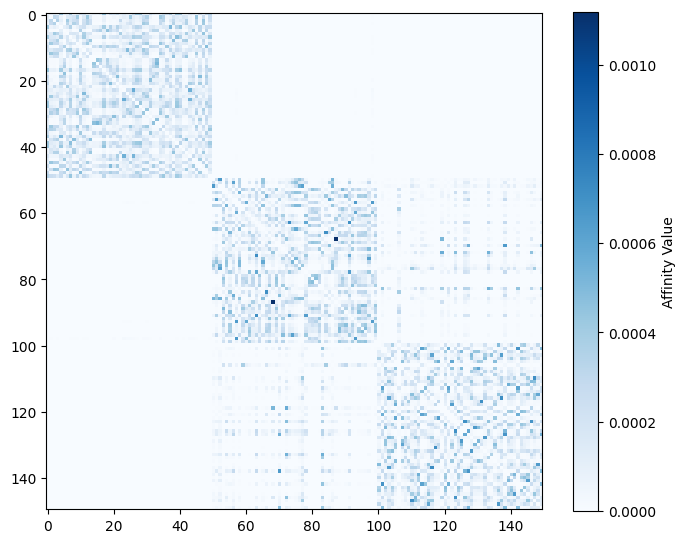
\includegraphics[width=0.7\linewidth]{figures/iris_affinity_matrix.png}
        \caption{Affinity values $p_{ij}$ of the Iris dataset visualized. The affinity matrix was generated using the standard perplexity value of 30.}
    %\end{center}
    \label{fig:iris_affinities}
\end{figure}

We can see the three clusters of the Iris dataset pretty clearly. 
From the visualization \ref{fig:iris_affinities}, it also seems like the first cluster is more well-defined than the second and third are. 
\textcolor{red}{If we run a dimensionality algorithm like PCA or t-SNE on it, we can also see that it performs well and clearly separates at least the first cluster from the other two.} 

So, it would seem that at least this first cluster would fulfil the condition that \begin{equation} p_{ij} \geq \frac{1}{10 N |\Omega(i)|} = \frac{1}{10 \cdot 150 \cdot 50} \end{equation}

However, when we investigate the $p_{ij}$ values of the first cluster (excluding, of course, the diagonal elements, since they are always zero), we notice that the smallest $p_{ij}$ value we observe is (rounded) $2.8 \cdot 10^{-7}$, whereas we calculated a lower bound of about $1.3 \cdot 10^{-5}$ above.
Furthermore, we calculated that a total number of 354 similarites between points in this same first cluster are smaller than the minimal $p_{ij}$ value required for it to be a cluster. 
Now, while \cite{LinStei22} do mention that there is some flexibility with respect to the exact constant being used - we would have to increase it by two orders of magnitude for this result to hold. 

For the last two clusters, we observe something even more interesting. 
If we consider the second cluster, we see that that the smallest similarity value between two points in it is $0.0$. 
This makes it virtually impossible to consider as a cluster, not matter how far we would scale the constant. 
One might argue that indeed clusters 2 and 3 belong together, but also then we observe some points having $0$ similarity to each other. 

\section{Initialization}
As mentioned above, the benefits of PCA initialization are well-studied (\textcolor{red}{include references here}). 
For example, \cite{kobak21} showed that t-SNE is better able to recover a synthetic 2D circle when initialized with PCA. 

Building on this work \textcolor{red}{and using their code (maybe I should cite the github here)}, we show that t-SNE also recovers other geometric structures like triangles (\ref{fig:triangle}) and squares (\ref{fig:square}) better when initialized with PCA. 

Implementation details: we sampled $n=7000$ points and added some Gaussian noise. We closely followed \cite{kobak21}, only changing the circle to a triangle and square. 

We also use two different seeds for each of the embeddings with random and PCA initialization. 
As expected, we see much more variance in the embedding when we use random initialization. While using PCA initialization eliminates some of this variance between embeddings, we can still observe small differences between the embeddings (especially of the triangle). 

\begin{figure}[h]
    \centering 
        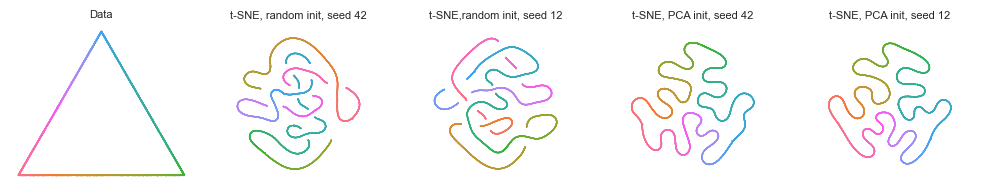
\includegraphics[width=\linewidth]{figures/t_sne_on_triangle.png}
        \caption{t-SNE on an equilateral triangle in 2D space. Using PCA initialization improves recovery of the structure better than when using random initialization.}
    \label{fig:triangle}
\end{figure}

\begin{figure}[h]
    \centering 
        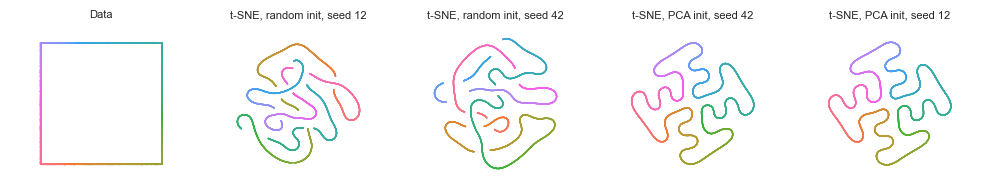
\includegraphics[width=\linewidth]{figures/t_sne_on_square.png}
        \caption{t-SNE performed on a square (with some Gaussian noise added) \textcolor{red}{the seeds of the first two embeddings here are switched up, it should be seed 42 first}}
    \label{fig:square}
\end{figure}

We thought it was interesting to see how PCA initialization helps with preserving geometric structures and to see that PCA-initialized t-SNE embeddings with different seeds still lead to slightly different results. 
But ultimately, it is well-established in the research that PCA should be used to initilize the low-dimensional embedding. 
We will therefore not conduct any other experiments regarding initialization. 

\textcolor{red}{TODO: think about if I want to say something about spectral initialization}

\section{Number of Iterations}
We ran t-SNE with a different number of iterations on the 4 datasets above. Our expectation was that bigger datasets need more iterations. The EE length was kept at 25 percent of the total number of iterations. 

\begin{figure}[h]
    \centering 
        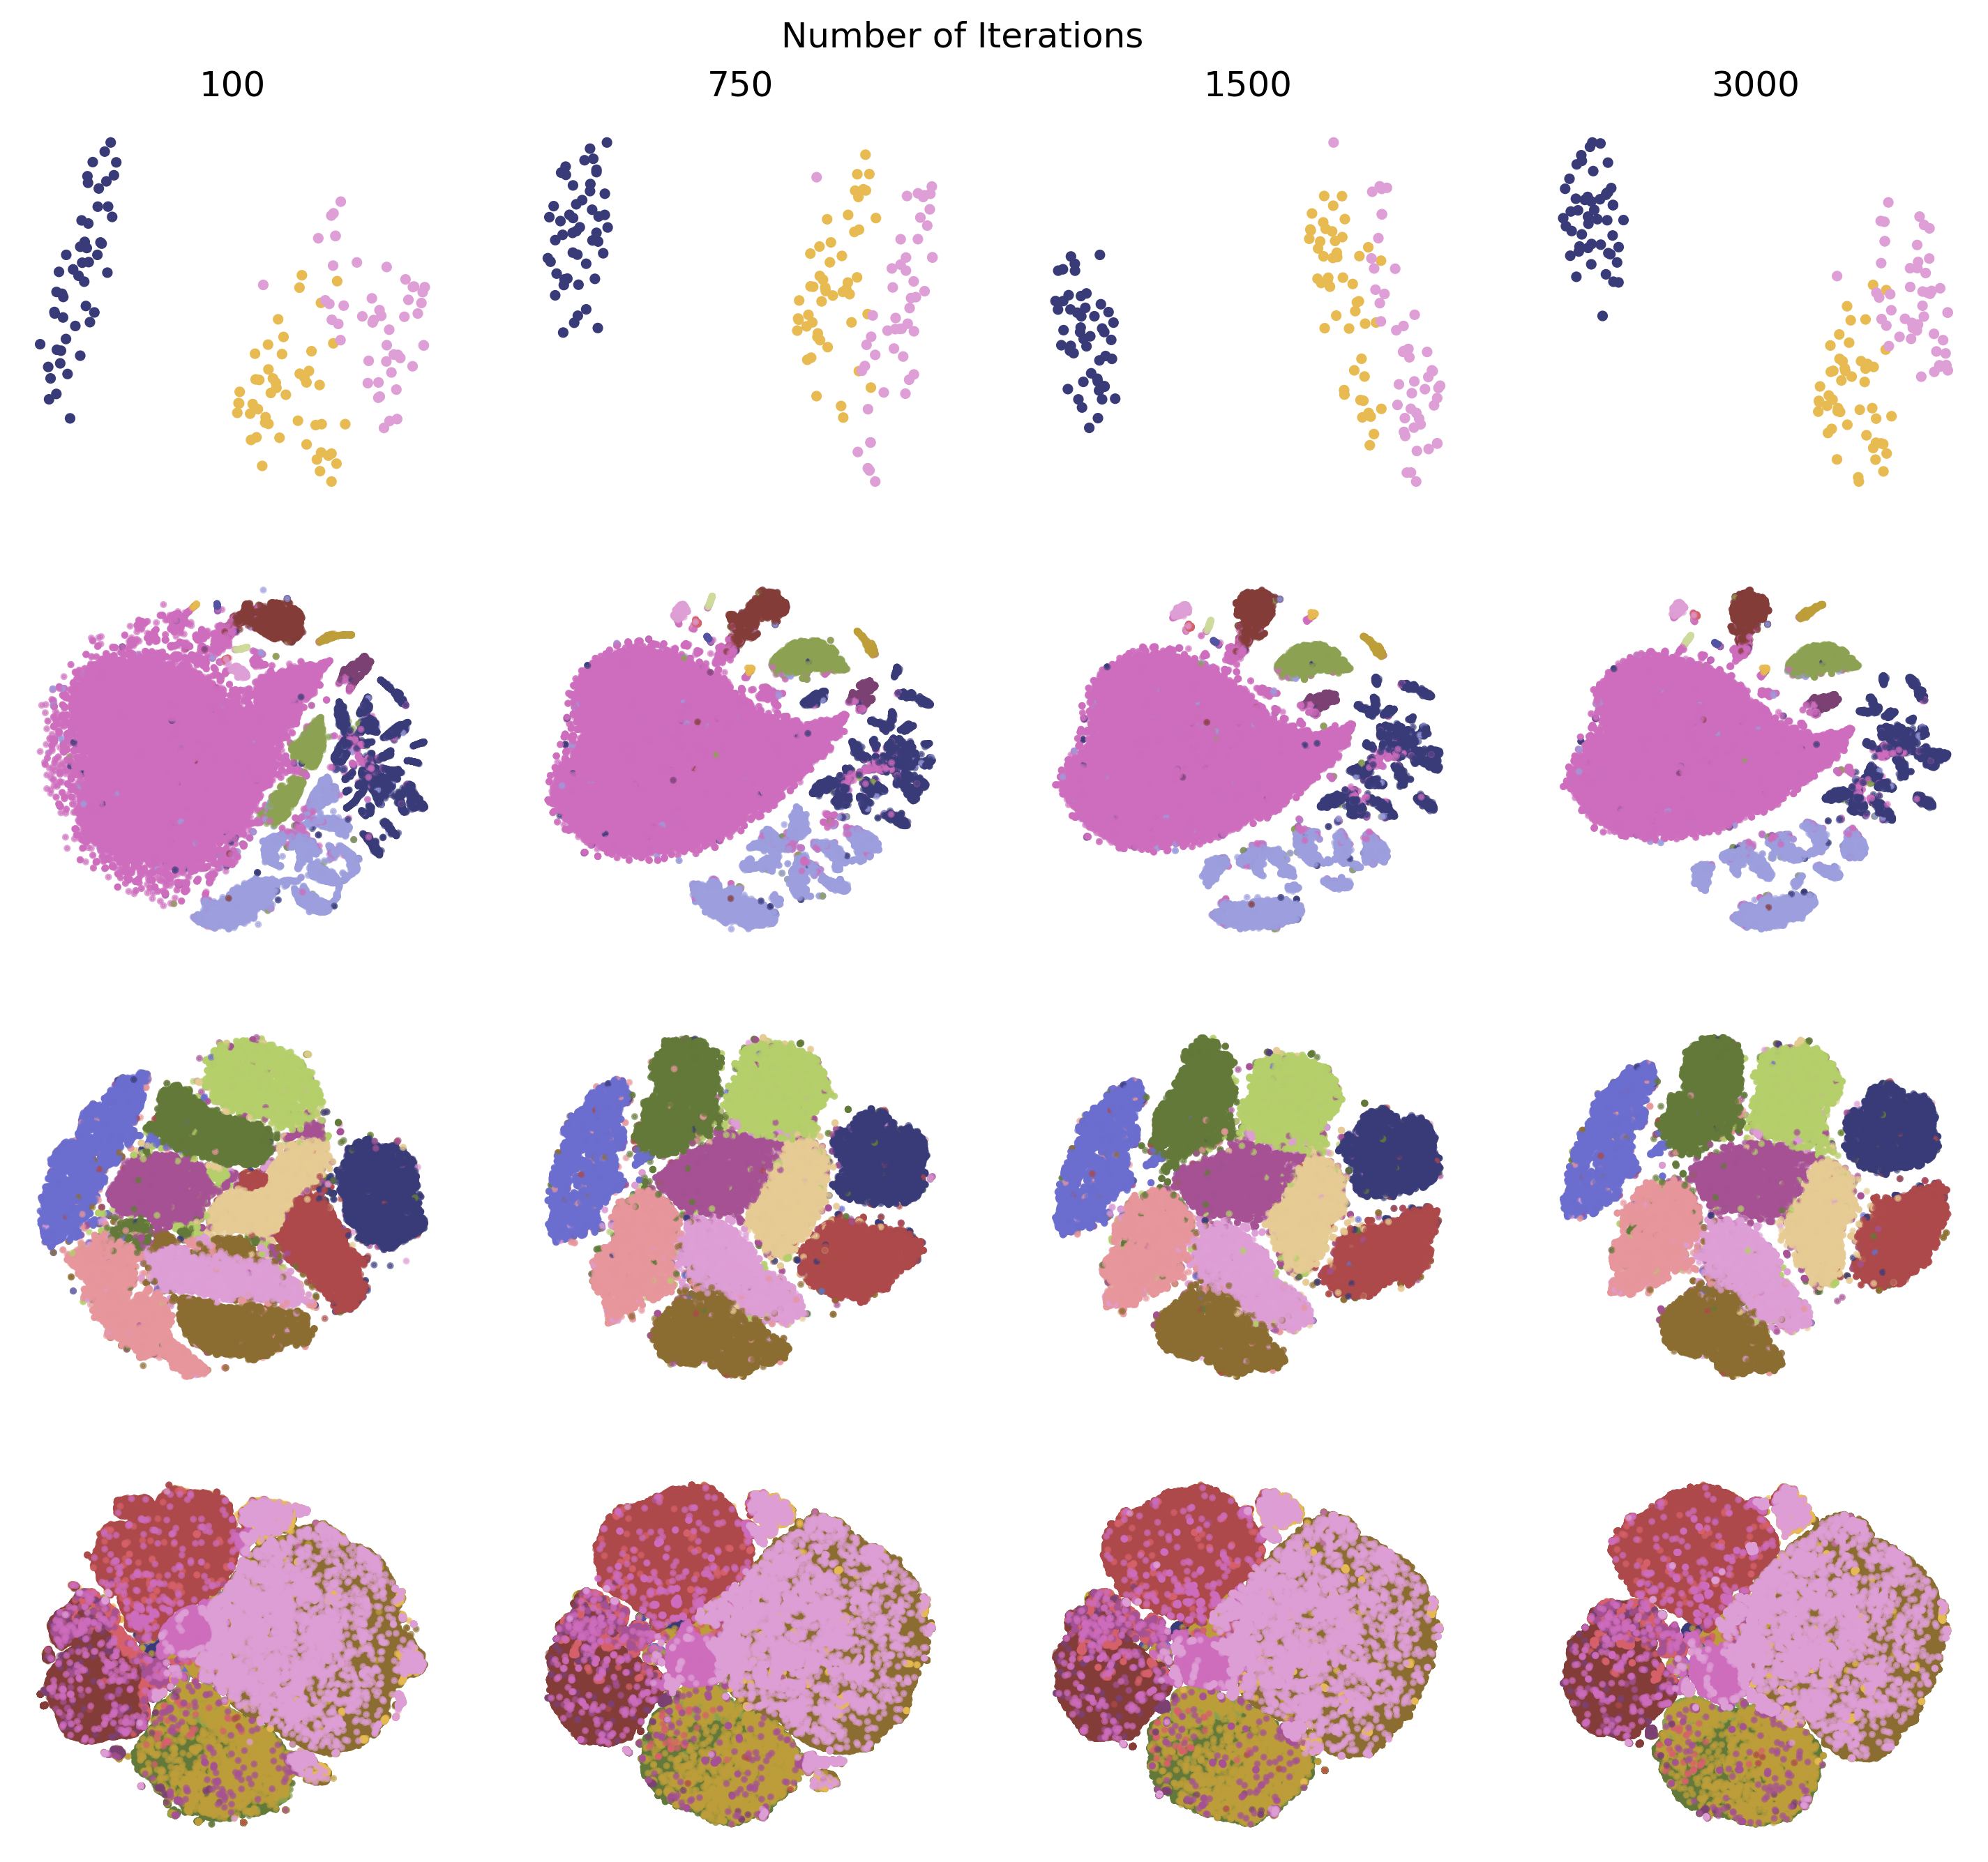
\includegraphics[width=\linewidth]{figures/n_iter/n_iter_embedding_grid_tab20b.png}
        \caption{Embeddings of the four datasets.}
    \label{fig:n_iter-grid}
\end{figure}

\begin{figure}[h]
    \centering 
        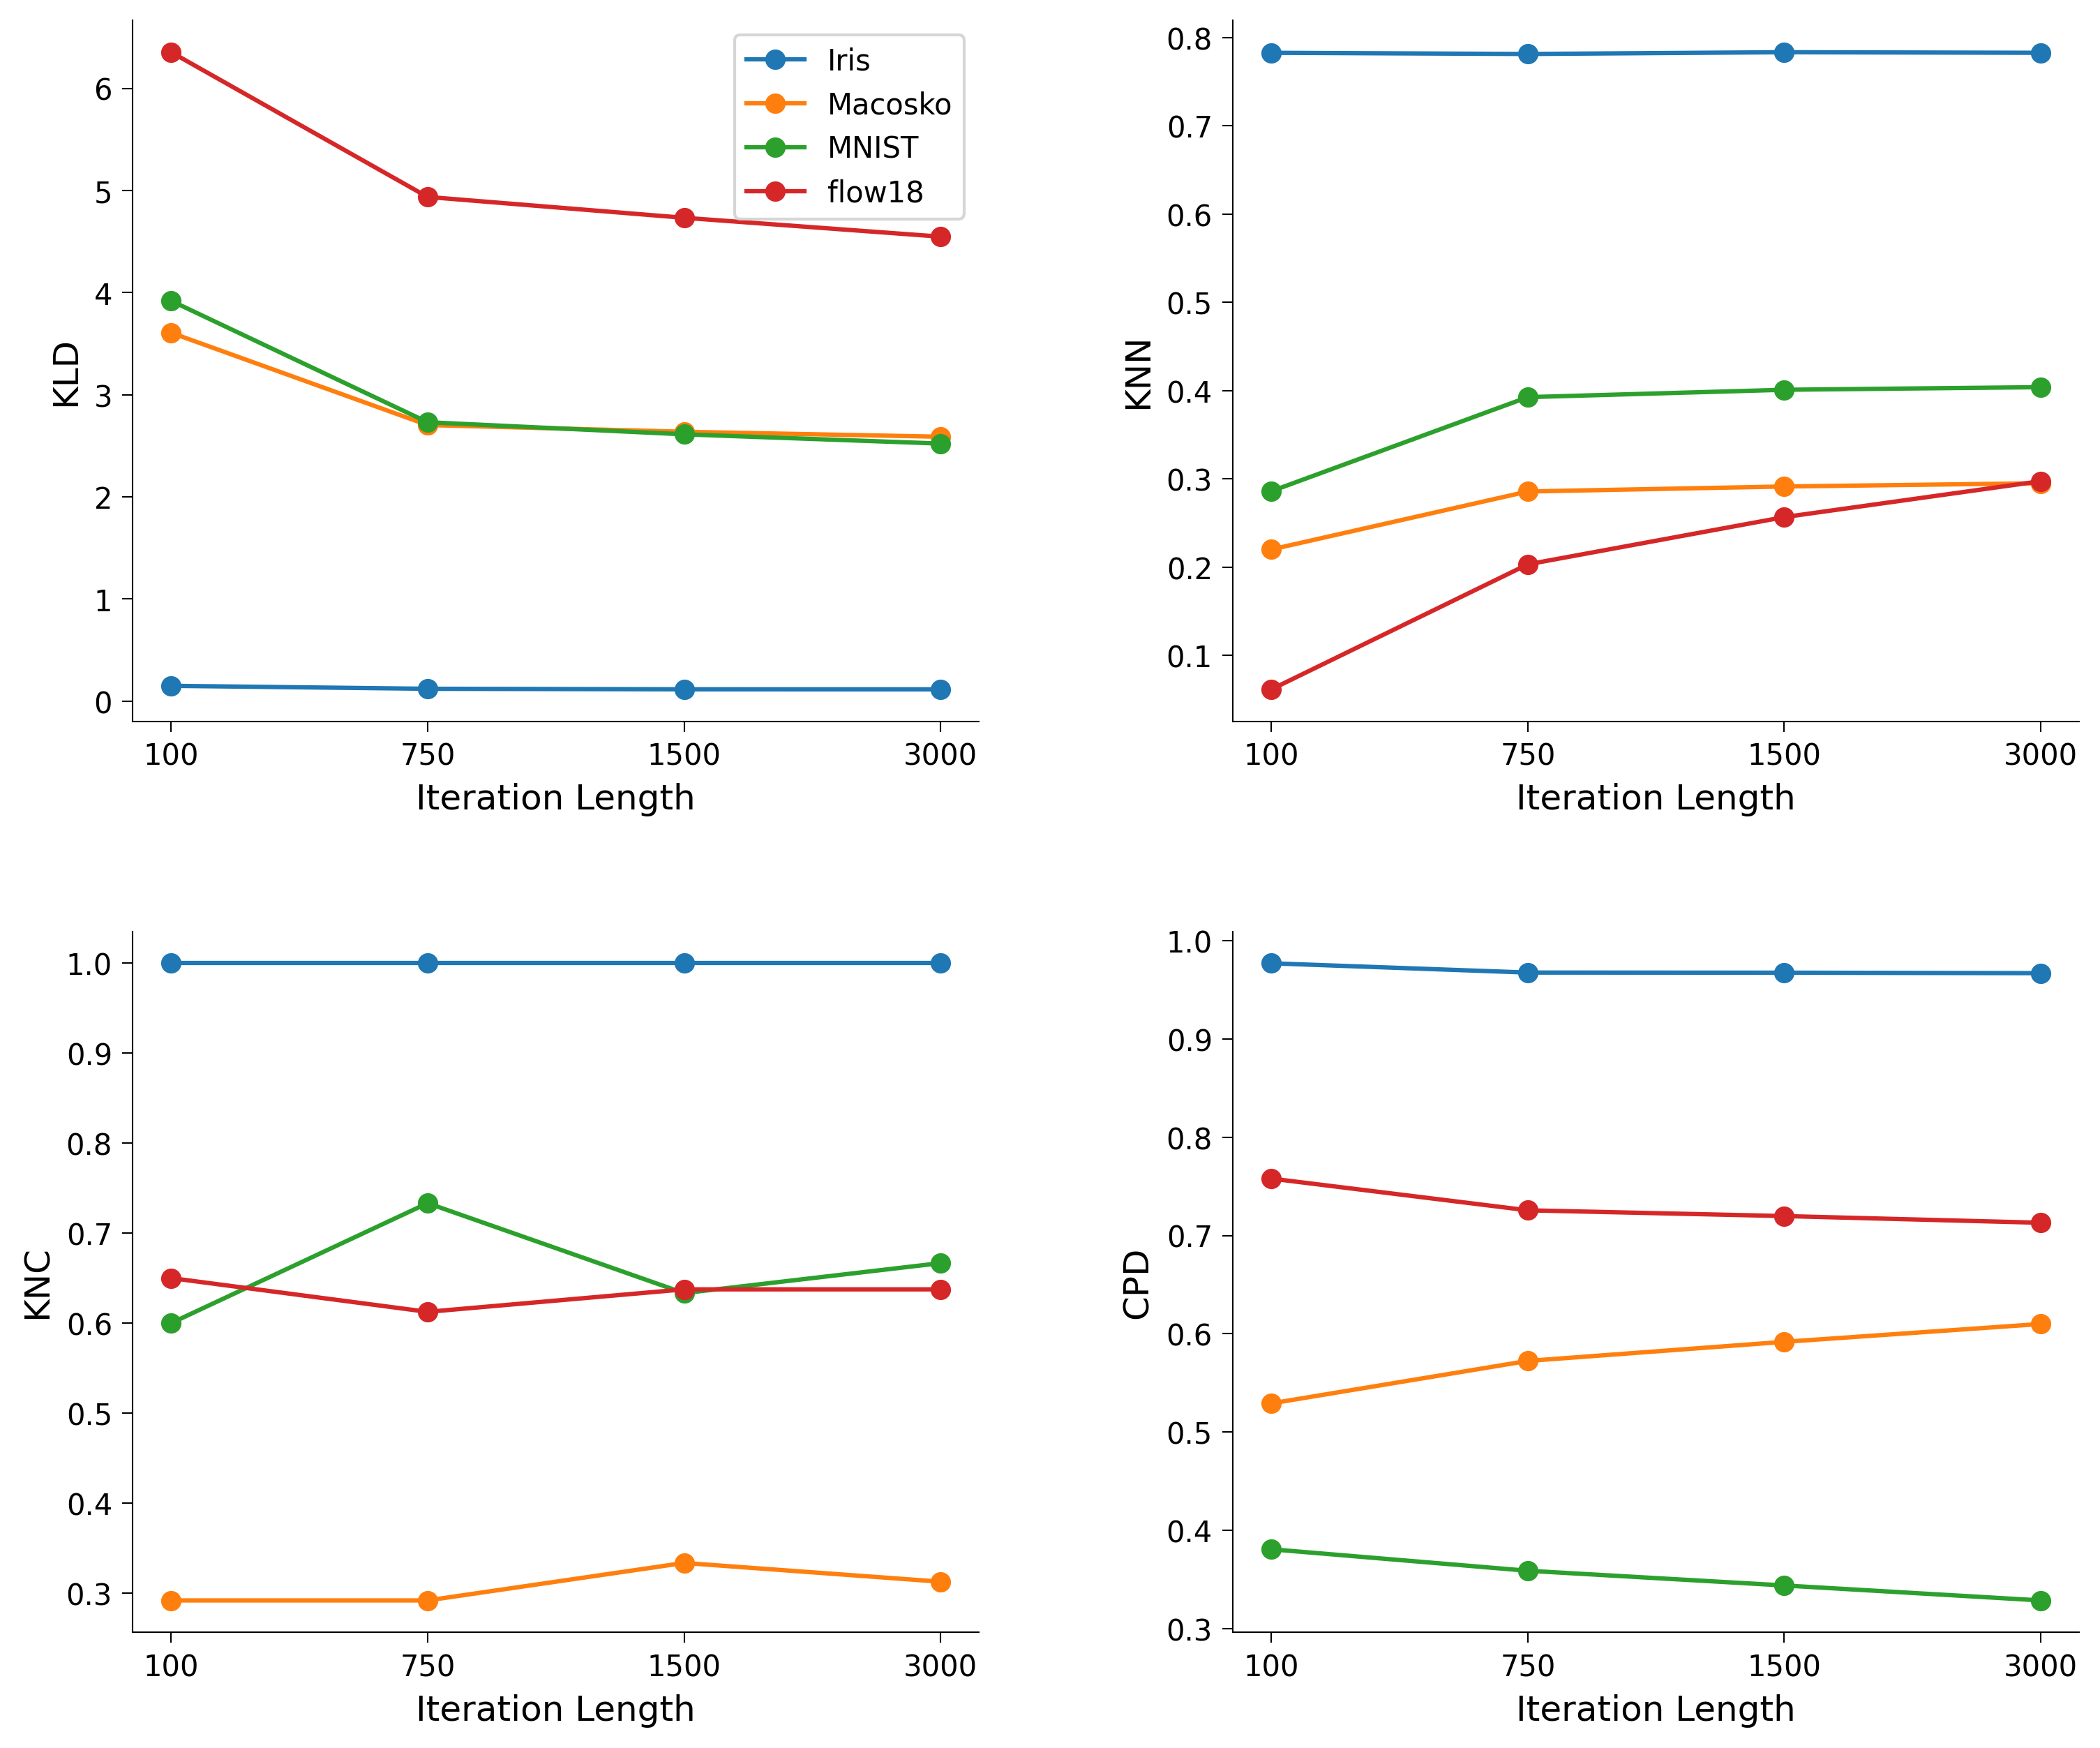
\includegraphics[width=\linewidth]{figures/n_iter/n_iter_4_quality_measures.png}
        \caption{quality measures. say what they show here.}
    \label{fig:n_iter-quality}
\end{figure}

We can observe that even 100 iterations is enough on the small Iris dataset. 
With 100 iterations, the embedding took 0.55 seconds to run, whereas the standard number of 750 iterations took 2.42 seconds. 
We also see that the largest dataset, Flow18, profits the most from the largest number of iterations, as expected. 

\section{An Implementation of Rescaled t-SNE for Large Data Limits}
For the Gaussian mixture data, we use $b=0.03$ and for MNIST $b=0.07$. In both cases $\kappa=15$ is used. 

\begin{figure}[h]
    \centering 
        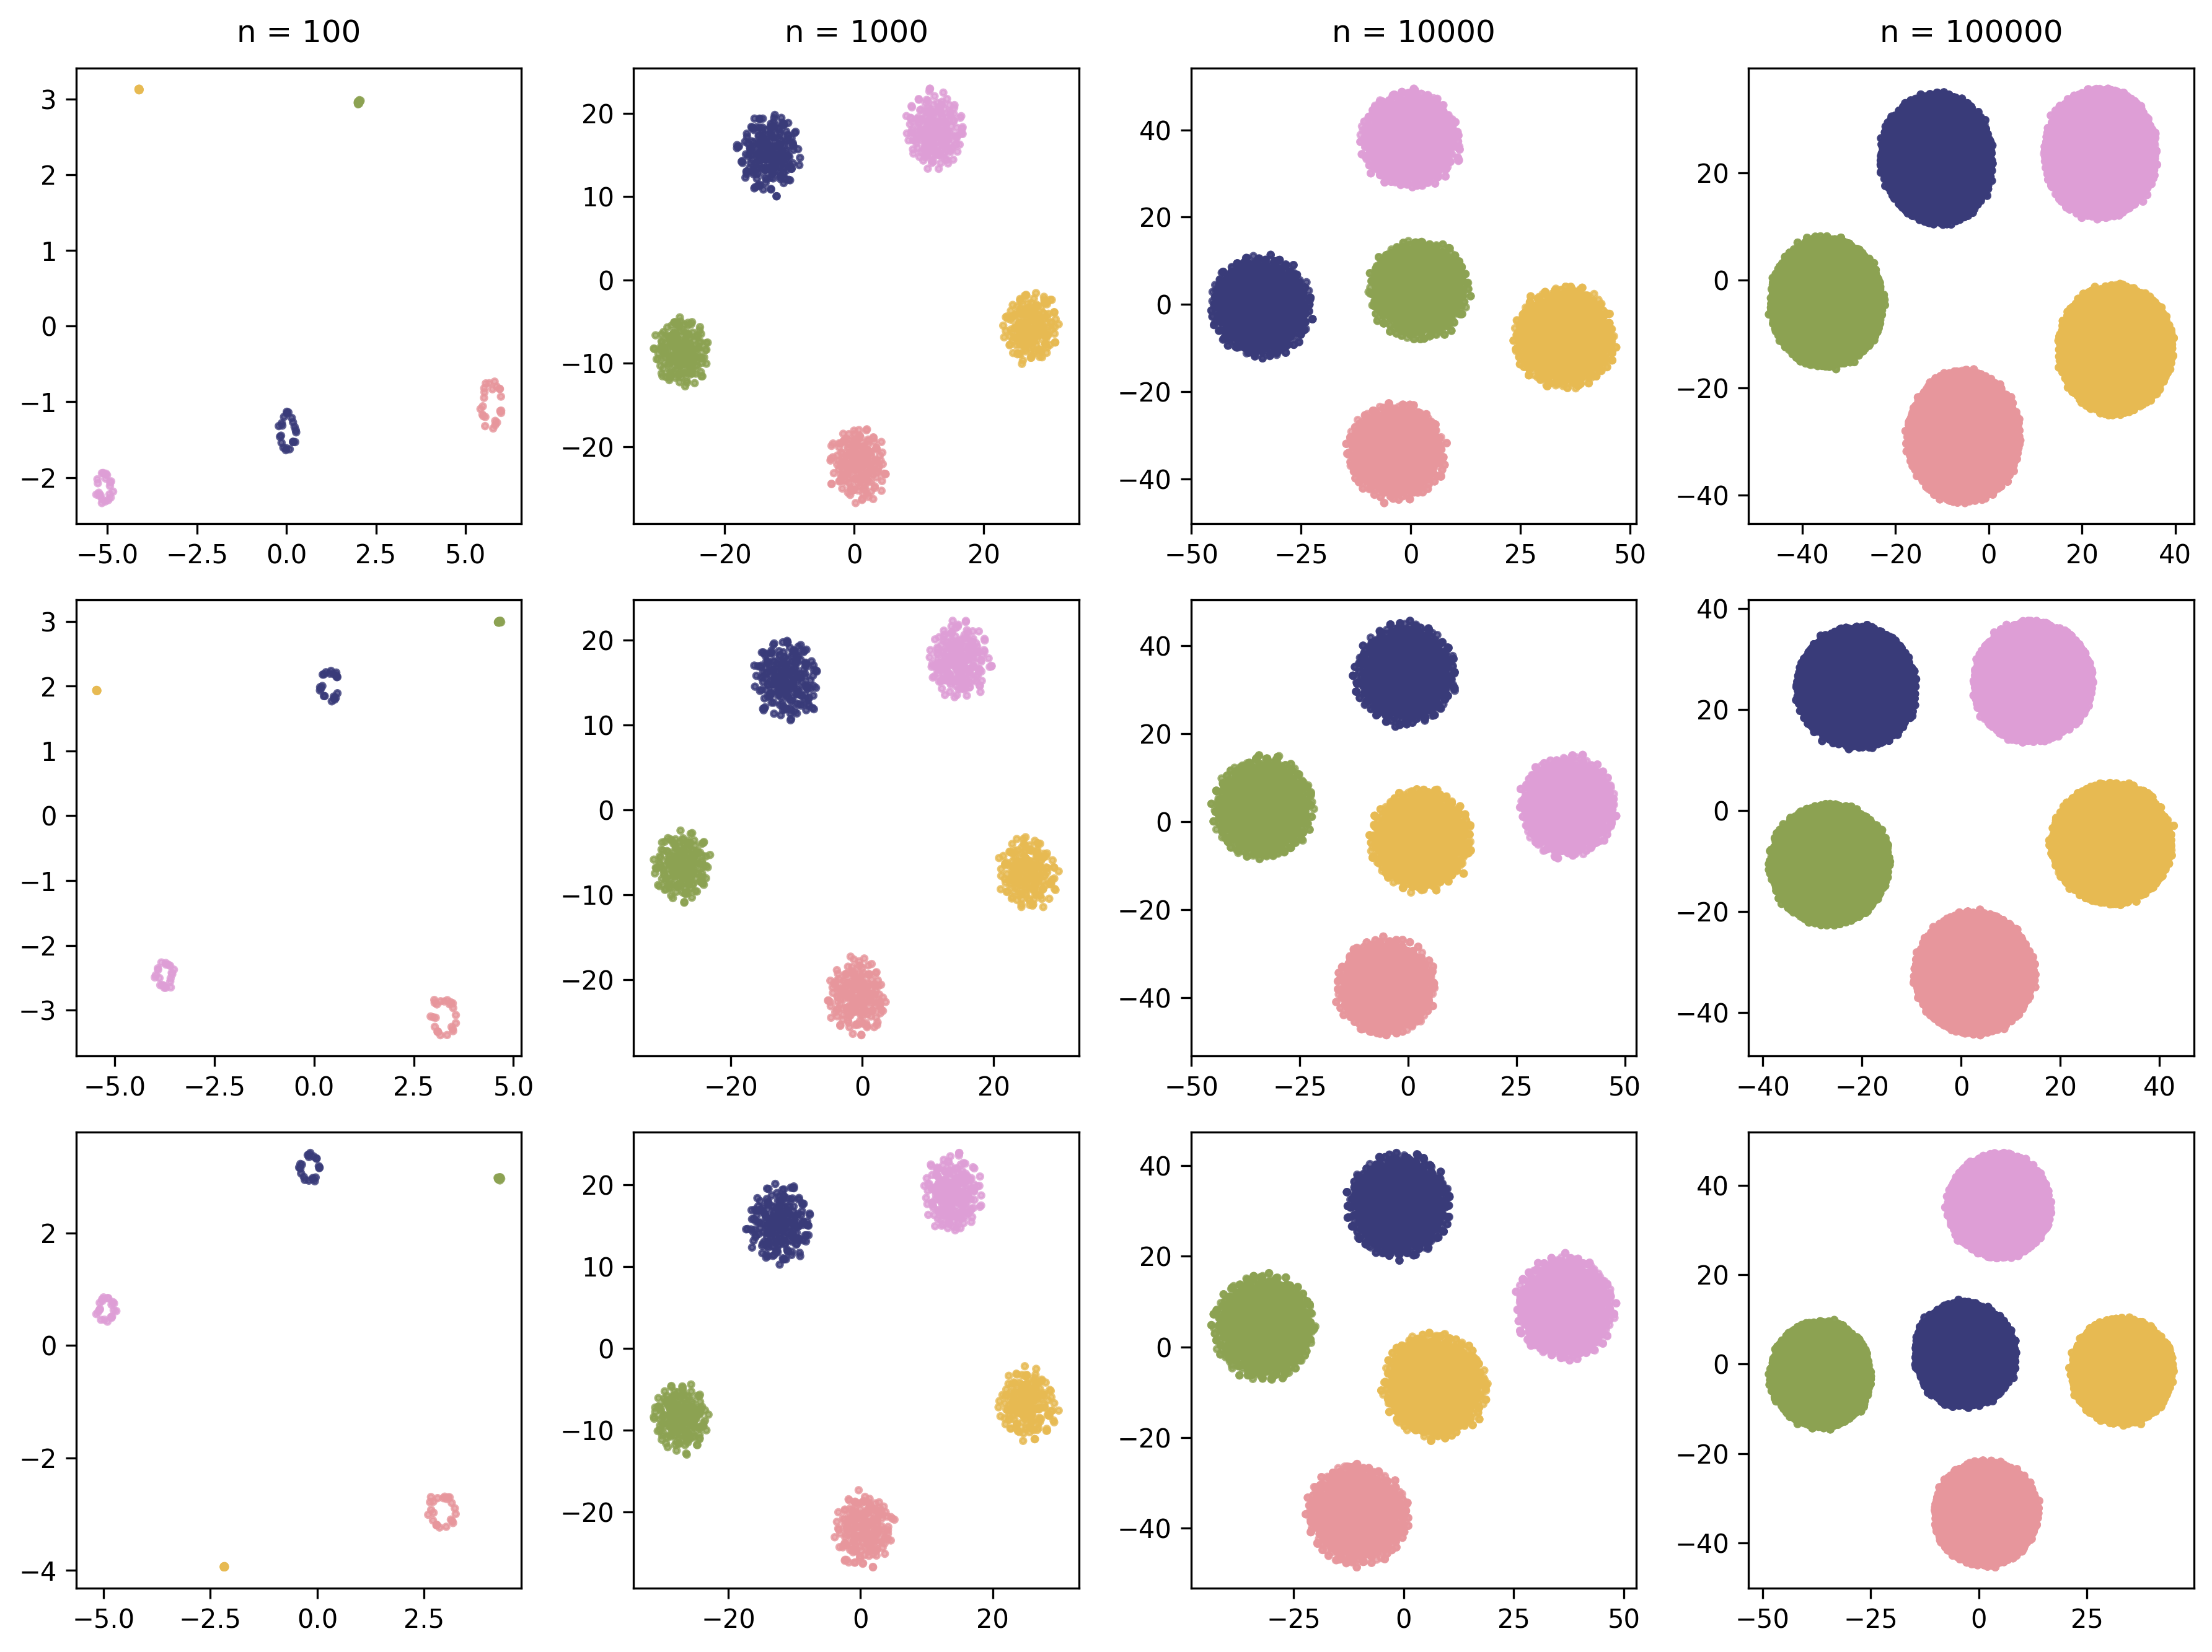
\includegraphics[width=\linewidth]{figures/rescaled/Gaussian_Mixture_standard_embedding_grid.png}
        \caption{Using standard t-SNE. Data generated from mixture of five Gaussian distributions.}
    \label{fig:Gaussian-standard}
\end{figure}

\begin{figure}[h]
    \centering 
        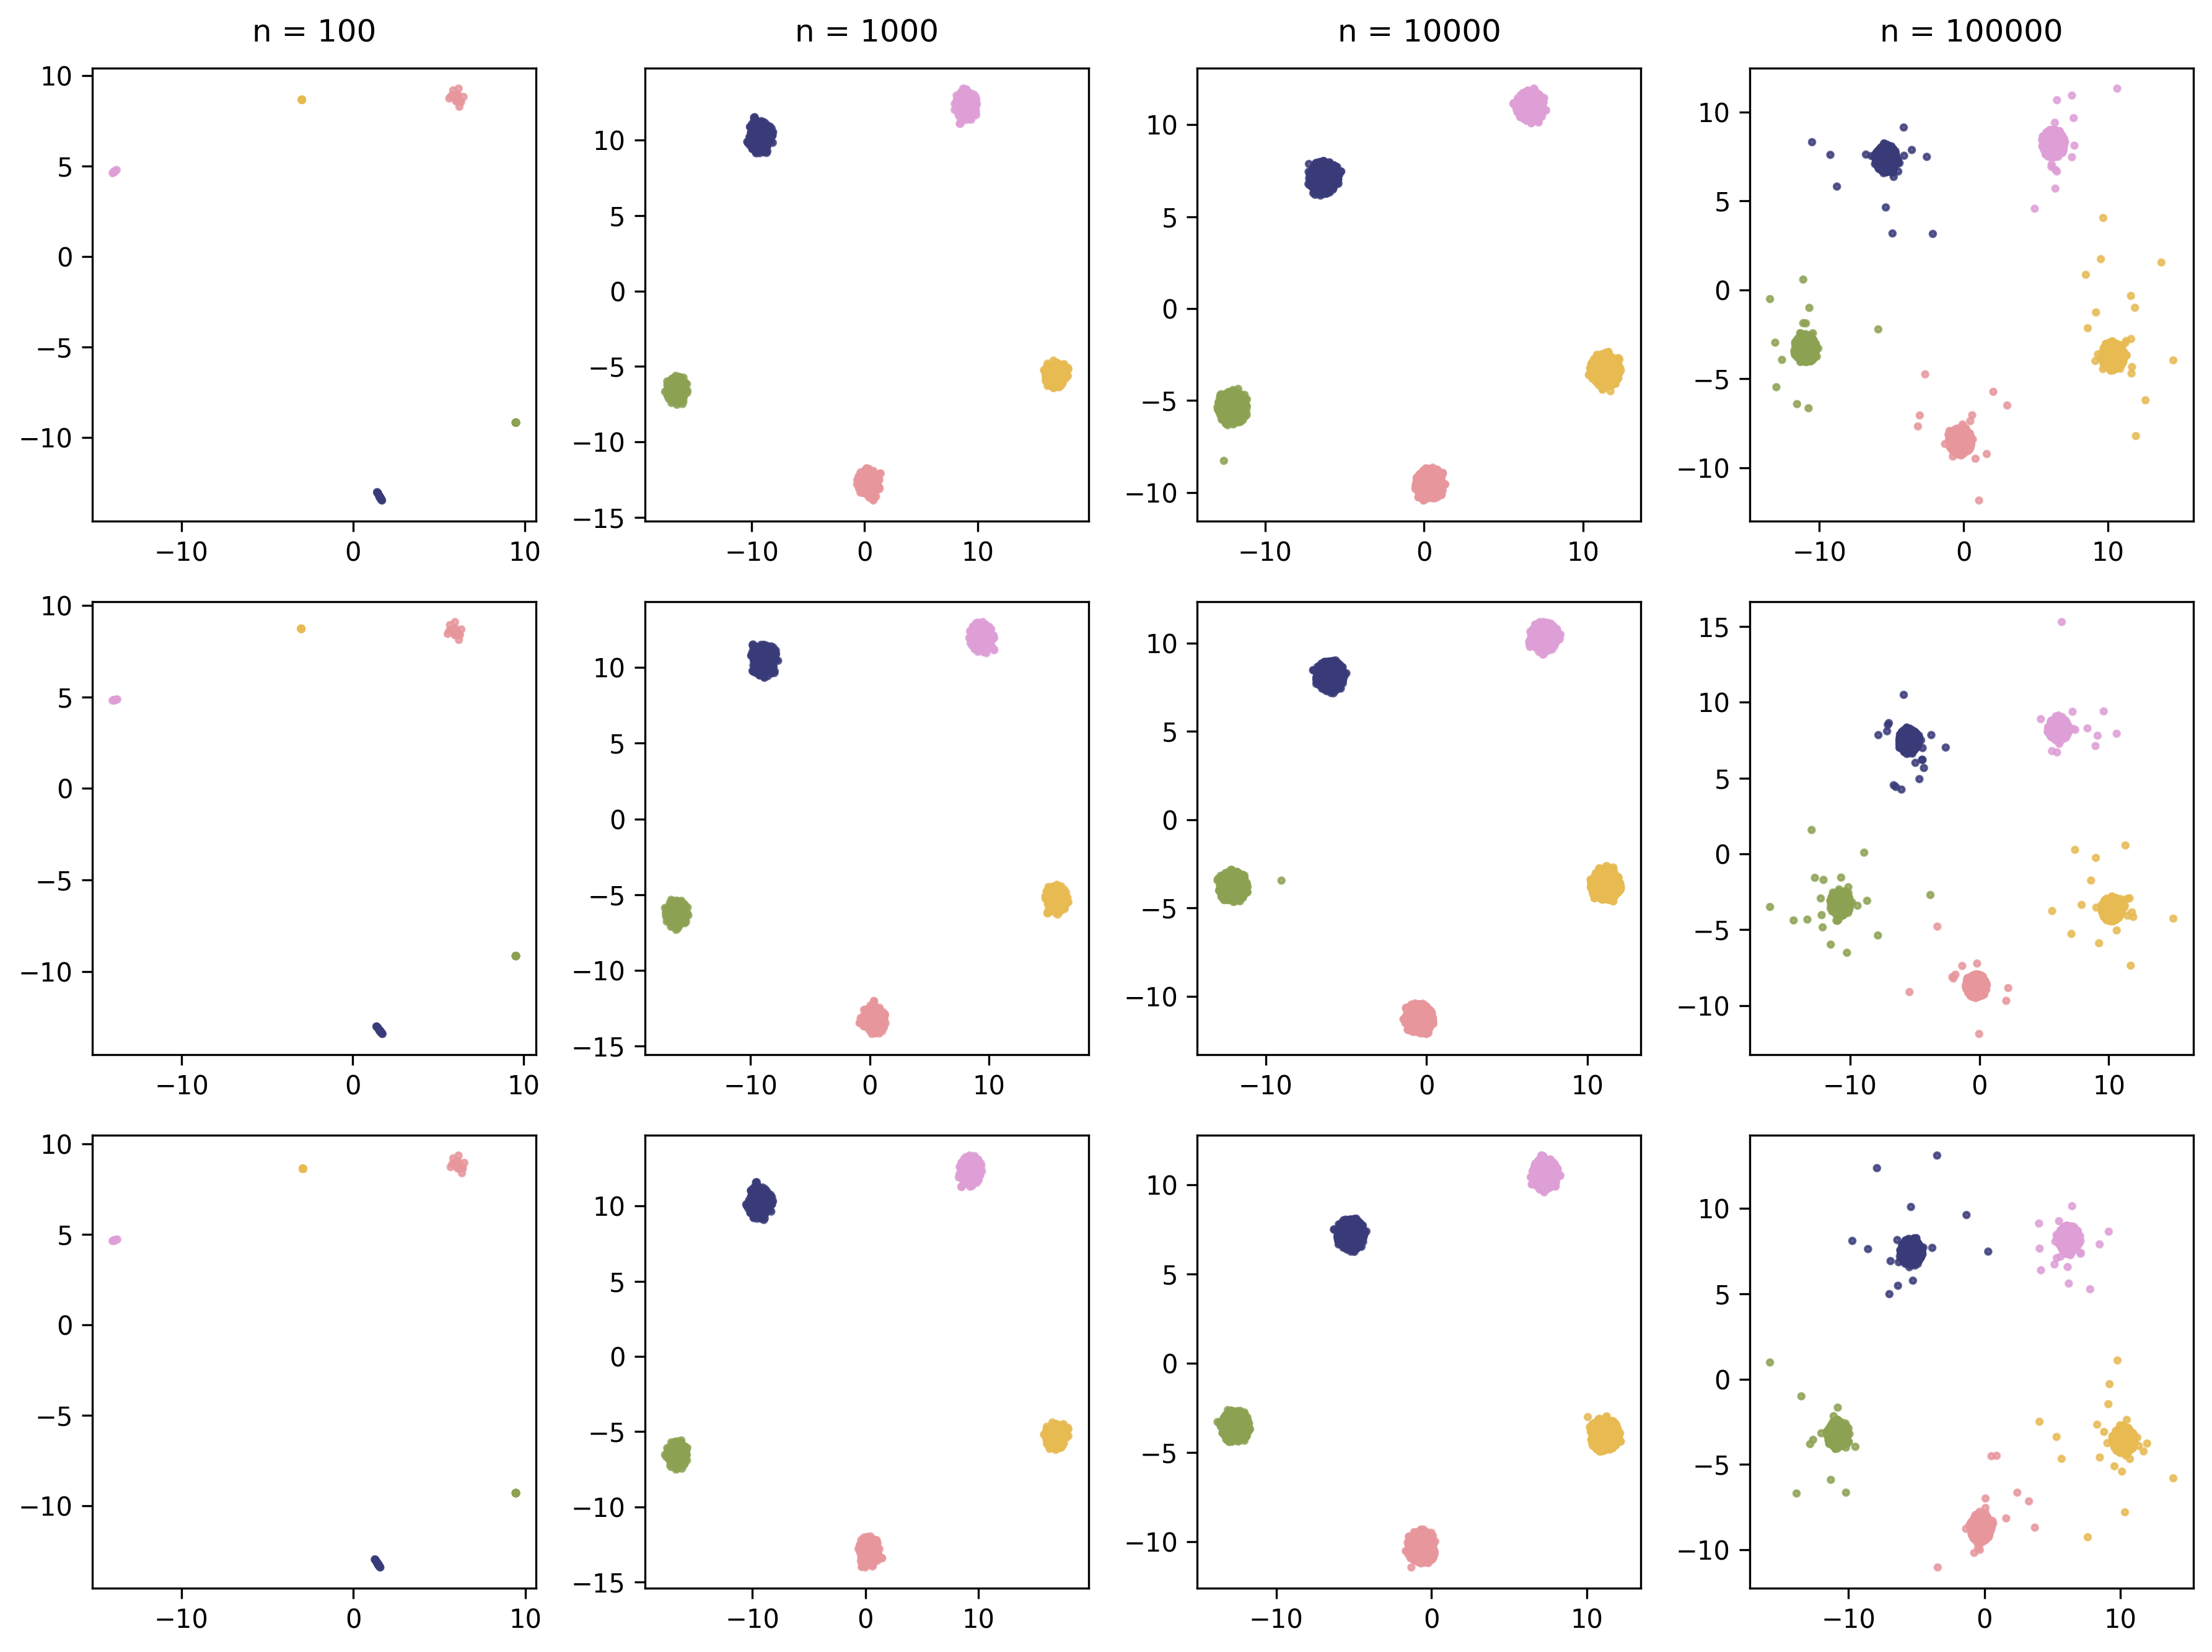
\includegraphics[width=\linewidth]{figures/rescaled/Gaussian_Mixture_rescaled_embedding_grid.png}
        \caption{Using rescaled t-SNE. Data generated from mixture of five Gaussian distributions.}
    \label{fig:Gaussian-rescaled}
\end{figure}

In the real world, things are more complicated. 

\begin{figure}[h]
    \centering 
        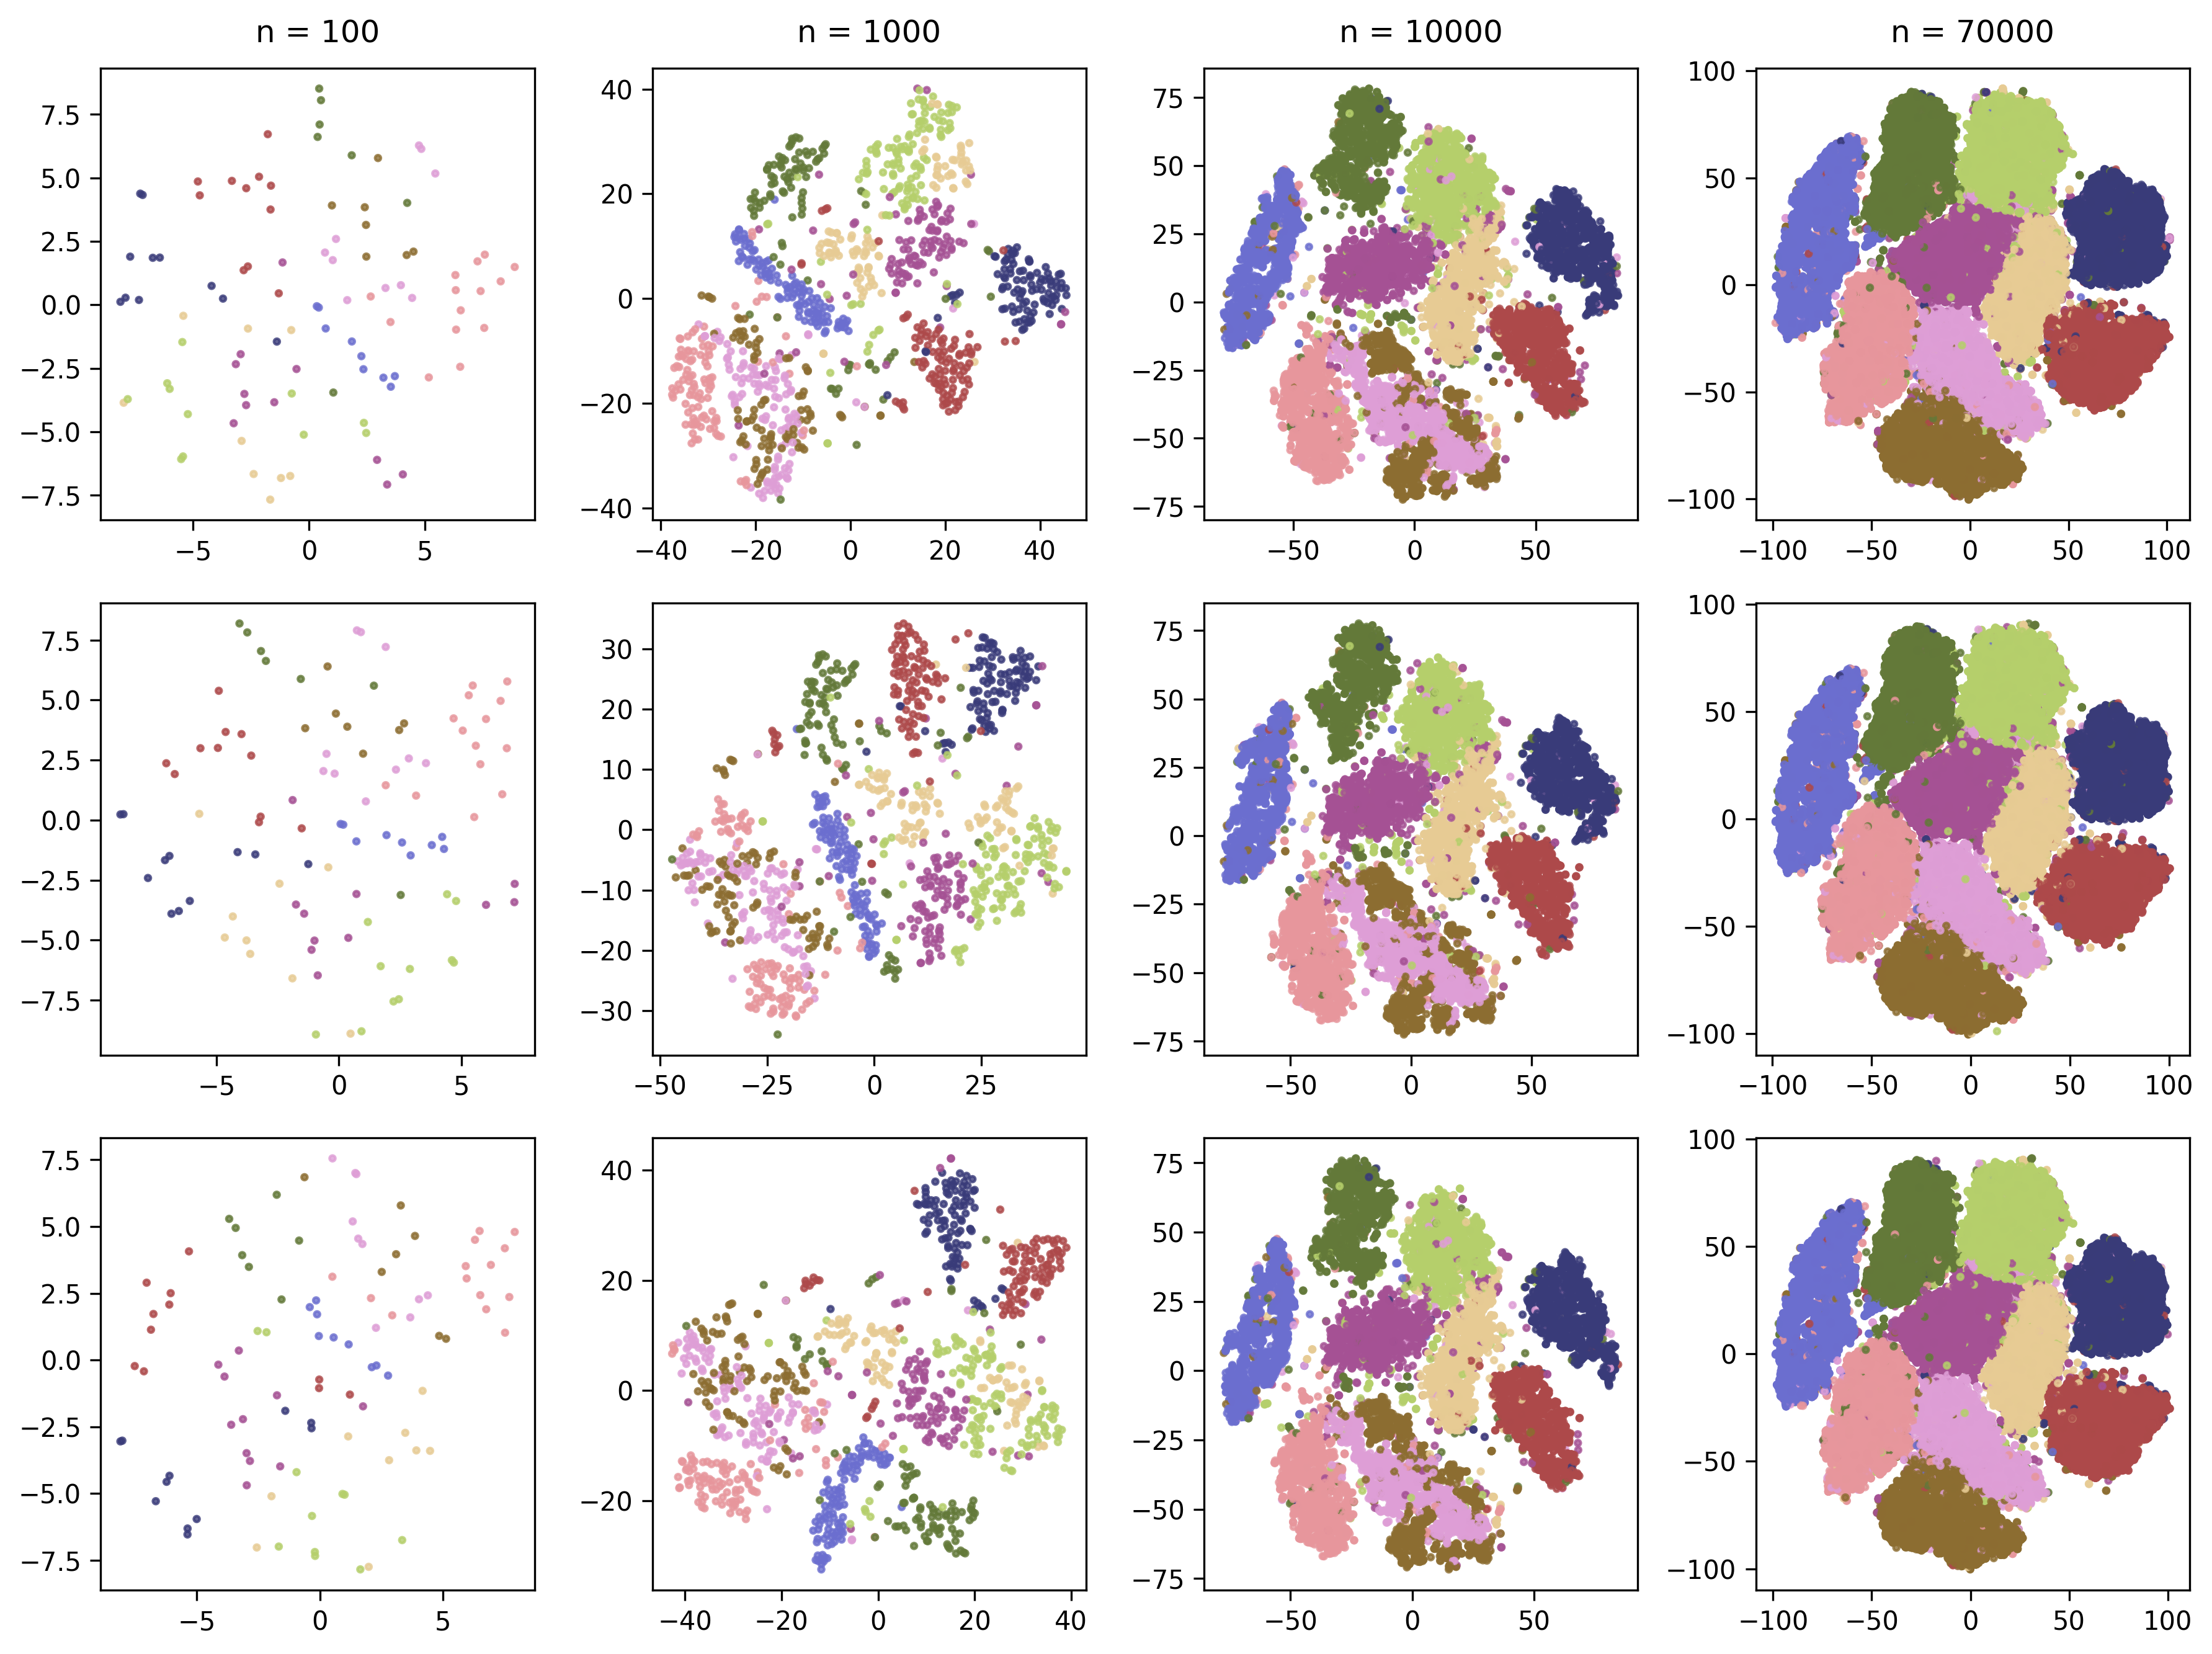
\includegraphics[width=\linewidth]{figures/rescaled/MNIST_standard_embedding_grid.png}
        \caption{Using standard t-SNE. Data sampled randomly from MNIST.}
    \label{fig:MNIST-standard}
\end{figure}

\begin{figure}[h]
    \centering 
        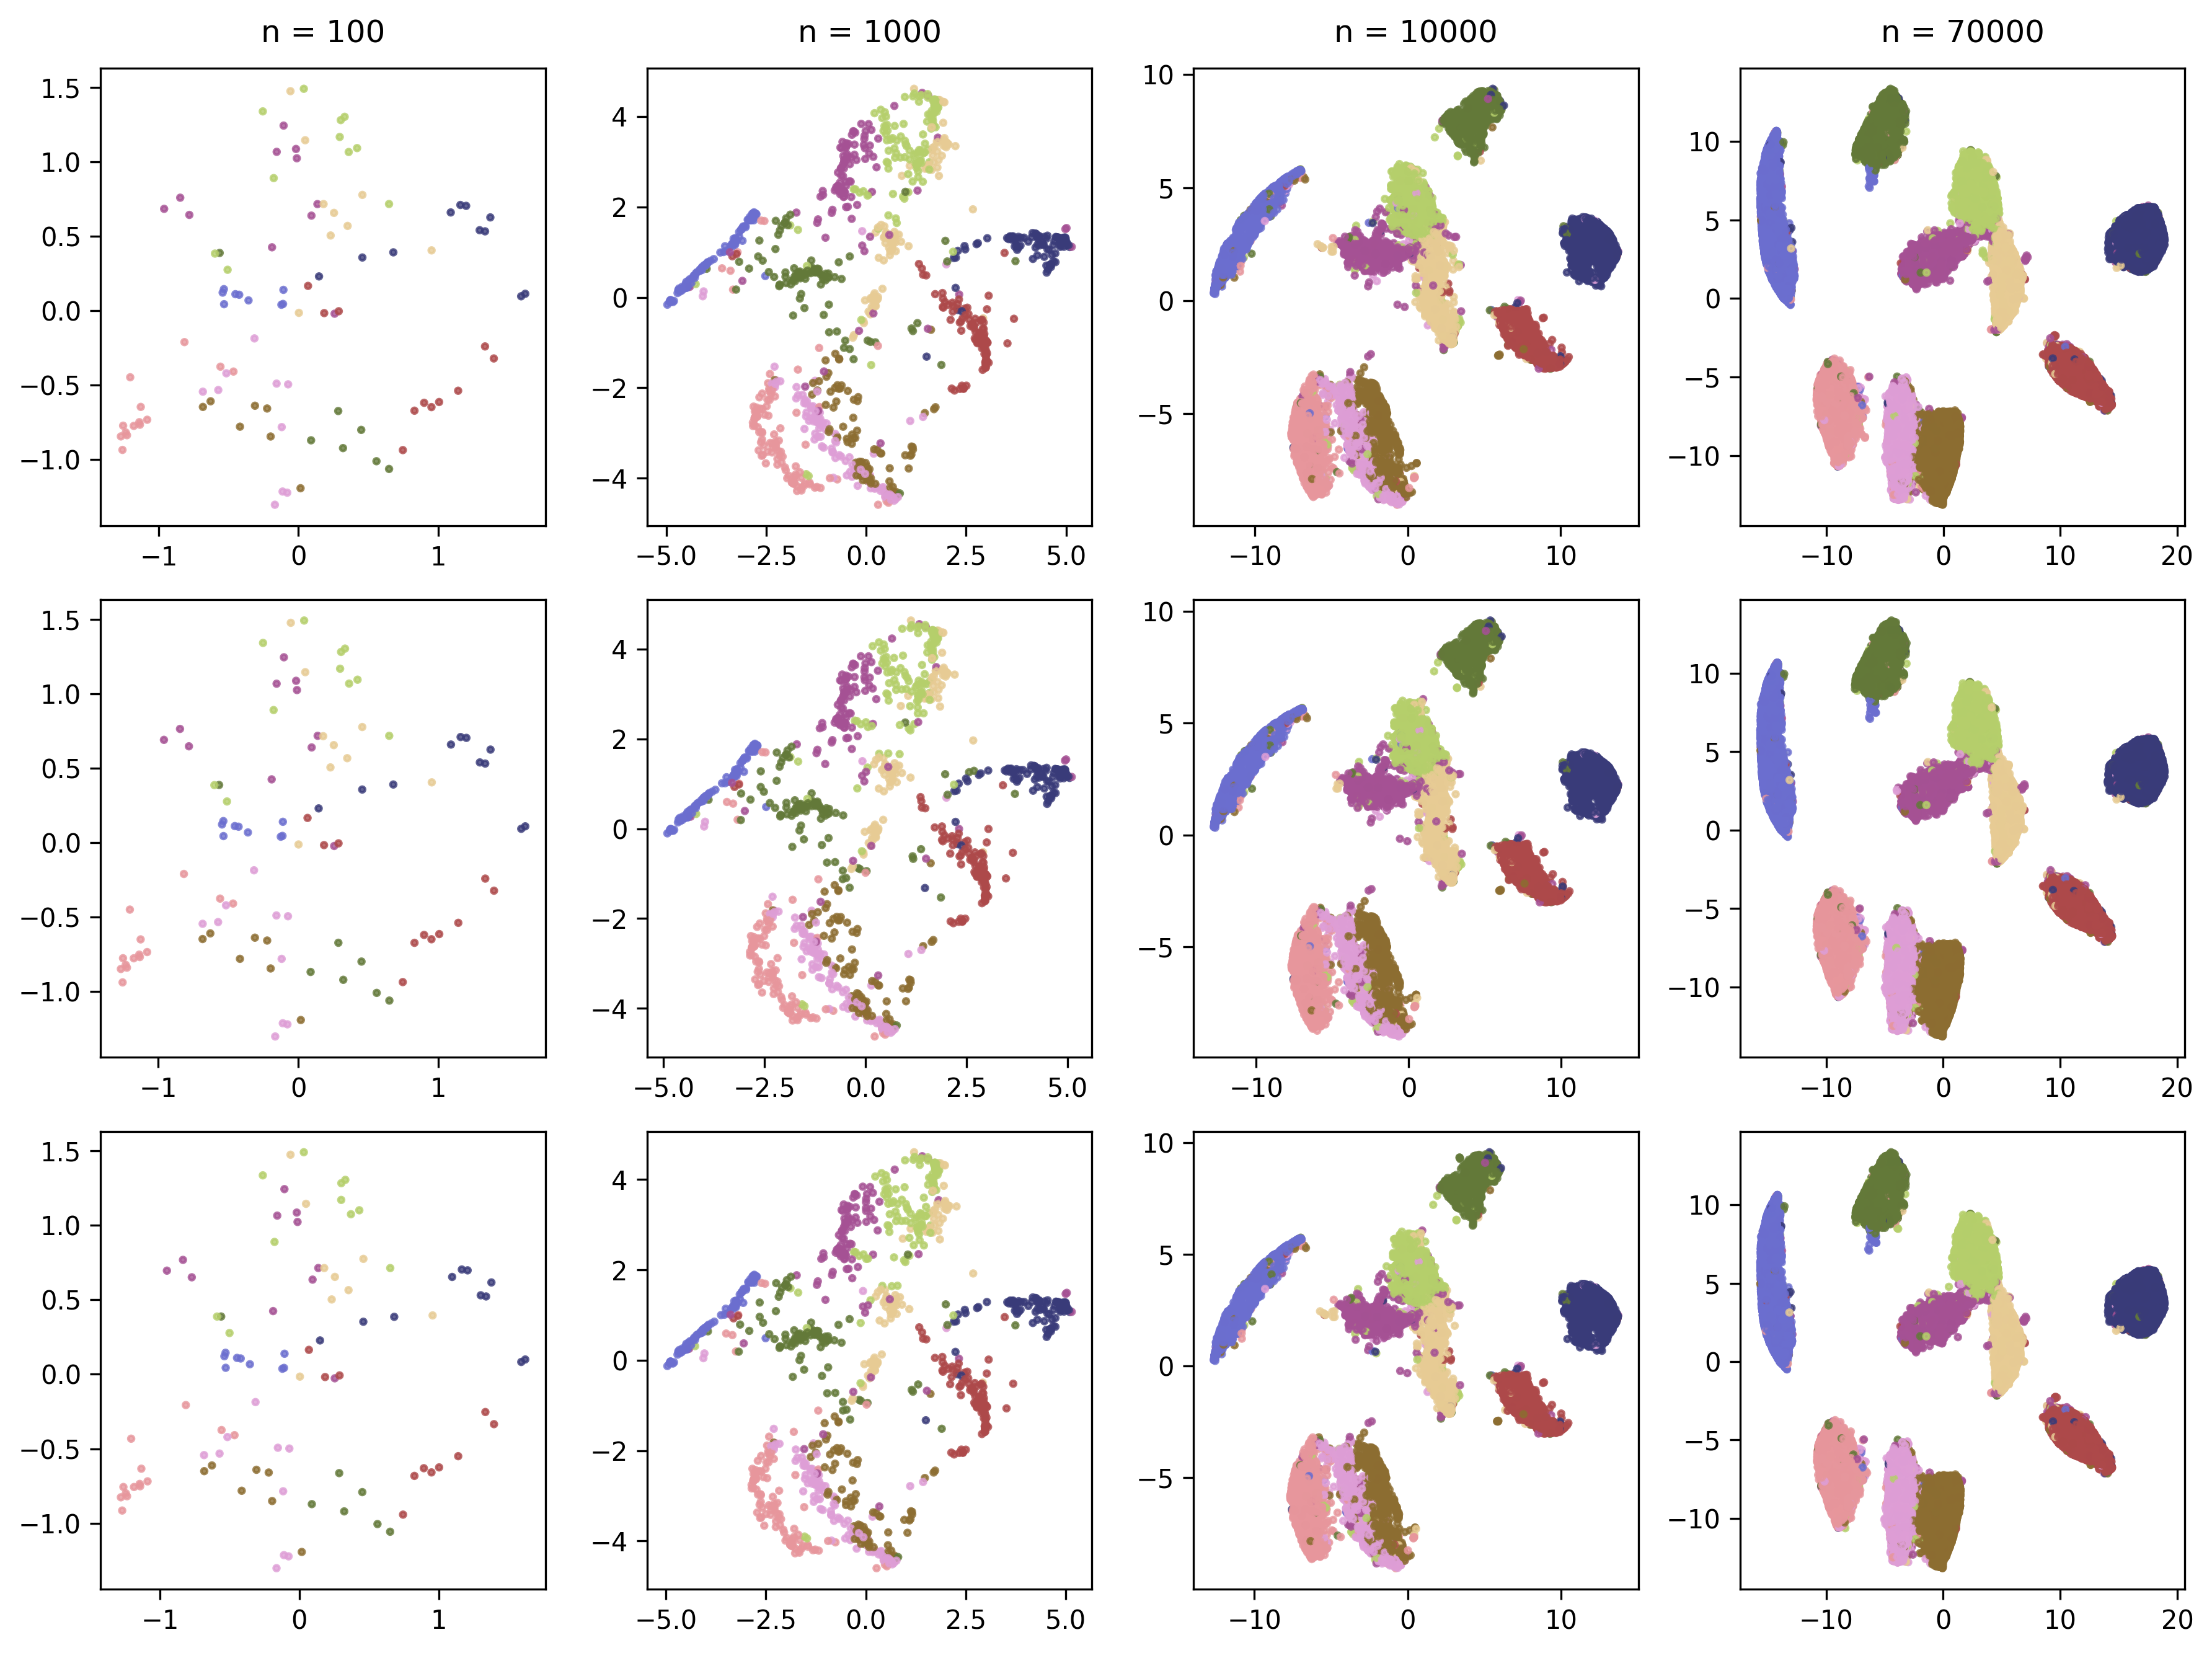
\includegraphics[width=\linewidth]{figures/rescaled/MNIST_rescaled_embedding_grid.png}
        \caption{Using rescaled t-SNE. Data sampled randomly from MNIST.}
    \label{fig:MNIST-rescaled}
\end{figure}

\section{Effect of Varying Perplexity Values}
there were some figures here before I removed them. 

\section{Early Exaggeration}
what effect does it have? 

\section{opt-SNE Implementation}
and comparison to default settings 